%\section{Power series and rational functions}
\begin{python0}
from solutions import *; clear() # -- clear solutions.tex
\end{python0}

A \defone{rational expression} is a fraction of polynomials:
\[
\frac{P(x)}{Q(x)}
\]
where $P(x)$ and $Q(x)$ are polynomials.
For instance
\[
\frac{x^{42} + 1}{5x^3 + 2x^2 + 67x}
\]
is a rational expression.
A \defone{rational function} is when you view the rational
expression as a function.
This is similar to polynomials.
You can write down a polynomial such as
\[
p(x) = x^2 + x + 1
\]
without ever evaluating it at $x = 2.5$ or any other $x \in \R$.
In that case, you are viewing $x^2 + x + 1$ as a
polynomial expression.
And if you compute $p(x)$ when $x \in \R$, then you are
viewing $p(x)$ as a polynomial function.
The distinction is not that important for us right now.
So I will view polynomials as expressions or functions
interchangeably.
Likewise I will use rational expressions and rational functions
interchangeably.
Note that a rational function is not defined at zeroes
of its denominator.
For instance $\frac{1}{(x-1)(x-2)}$ as a rational function
is not defined at $x = 1, 2$.

Here are some formulas that translate between certain power series and rational 
functions.
For $x \in \R$ with $|x| < 1$, we have the following:
\begin{enumerate}
\item[]\textsc{Geometric series}
\[
\frac{1}{1-x} = \sum_{n=0}^\infty x^n 
\]
\item[]\textsc{Power of geometric series}
\[
\biggl(
\frac{1}{1-x}
\biggr)^k
 = \sum_{n=0}^\infty \binom{k+n-1}{n} x^n 
\]
\end{enumerate}

Note the requirement that $|x| < 1$.
This number \lq\lq1" is called the \defone{radius of convergence} of $1/(1-x)$.
For instance for $x = 1/2$, since $|x| = |1/2| < 1$, i.e., I would say that $x=1/2$ is
\lq\lq in the radius of convergence",
\[
\sum_{n=0}^\infty x^n = \sum_{n=0}^\infty (1/2)^n = 1 + 1/2 + 1/4 + 1/8 + \cdots
\]
and if you have time and compute 1000 terms, $1 + 1/2 + 1/4 + 1/8 + \cdots + 1/2^{999}$
will be very close to $1/(1 - (1/2)) = 2$.
And if you compute $1 + 1/2 + 1/4 + 1/8 + \cdots + 1/2^{999999}$, you'll see that it will be even closer to $2$.
We say that $\sum_{n=0}^\infty (1/2)^n$ is
\defterm{convergent}\tinysidebar{convergent \\ converges}\index{convergent}
and it
\defterm{converges}\index{converges}
to $2$.
For instance the geometric series formula does not even make sense when $x = 1$ since
\[
\frac{1}{1 - x} = \frac{1}{1 - 1}  = \frac{1}{0}
\]
is not defined and
\[
\sum_{n=0}^\infty x^n = \sum_{n=0}^\infty 1^n  = 1 + 1 + 1 + 1 + \cdots
\]
blows up to infinity!
And when $x$ is beyond the radius of convergence, say $x = 10$, then
\[
\frac{1}{1 - x} = \frac{1}{1 - 10}  = -\frac{1}{9}
\]
is defined while
\[
\sum_{n=0}^\infty x^n = \sum_{n=0}^\infty 10^n  = 1 + 10 + 100 + 1000 + \cdots
\]
blows up to infinity.

(\textsc{Aside.}
In general, for a power series $f(x) =\sum_{n=0}^\infty a_nx^n$,
there is the concept of the radius of convergence, $R$, of $f(x)$.
Assuming $R$ exists and is finite,
if $|x| < R$, $f(x)$ converges to some
real number and if $|x| > R$, $f(x)$ diverges.
More details in Calculus.)

Note that (b) includes (a) (when $k=1$).
Note also that the $x$ appears in the above as a variable.
In particular on replacing $x$ in (a) with $4x$ you can
\[
\frac{1}{1-4x} = \sum_{n=0}^\infty (4x)^n = \sum_{n=0}^\infty 4^n x^n 
\]
Note that in this case the equality holds for $x \in \R$ such that
\[
|4x| < 1
\]
i.e., when
\[
|x| < 1/4
\]
So I would say that the radius of convergence of $\sum_{n=0}^\infty 4^n x^n$ is $1/4$.

You can also handle this:
\[
\frac{1}{3-x}
\]
All you need to do is to force the 3 to become 1 like this:
\[
\frac{1}{3-x} 
= \frac{1}{3} \cdot \frac{1}{1 - x/3}
\]
In this case the radius of convergence is $1/3$, i.e., you should only
substitute values of $x \in \R$ into the power series if $|x/3| < 1$,
i.e., $|x| < 3$.
And for $|x| < 3$, you get
\begin{align*}
\frac{1}{3-x} 
&= \frac{1}{3} \cdot \frac{1}{1 - x/3} \\
&= \frac{1}{3} \sum_{n=0}^\infty \biggl( \frac{x}{3} \biggr)^n \\
&= \sum_{n=0}^\infty \frac{1}{3} \biggl( \frac{1}{3} \biggr)^n x^n \\
&= \sum_{n=0}^\infty \frac{1}{3^{n+1}} x^n
\end{align*}

And if you have a $+$ instead of a $-$:
\[
\frac{1}{3+x} 
\]
you just force a $-$ to appear:
\[
\frac{1}{3+x} 
= \frac{1}{3 - (-x)}
\]
and then proceed as above:
\begin{align*}
\frac{1}{3+x} 
&= \frac{1}{3 - (-x)} \\
&= \frac{1}{3} \cdot \frac{1}{1 - (-x/3)}
\end{align*}
At this point, to compute the radius of convergence, use $|-x/3| < 1$ to get
$|x| < 3$.
Continuing the above, if $|x| < 3$,
\begin{align*}
\frac{1}{3+x} 
&= \frac{1}{3} \cdot \frac{1}{1 - (-x/3)} \\
&= \frac{1}{3} \sum_{n=0}^\infty \biggl( \frac{-x}{3} \biggr)^n \\
&= \sum_{n=0}^\infty (-1)^n \frac{1}{3^{n+1}} x^n
\end{align*}

Whenever you're doing computations,
it's always a good idea to check your work.
In the case of series, it is easy to write simple programs to
verify your computations or by doing some computations by hand.
For instance the above computations claim that
\begin{align*}
\frac{1}{3+x} 
&= \sum_{n=0}^\infty (-1)^n \frac{1}{3^{n+1}} x^n \tag{$*$}
\end{align*}
So let's choose a value for $x$ and see if the 
right side of the identity equals the left.
For this case, the radius of convergence is $|x| < 3$.
Of course the easiest number to use is $x = 0$.
When $x = 0$,
\begin{align*}
\frac{1}{3 + x} &= \frac{1}{3} \\
\sum_{n=0}^\infty (-1)^n \frac{1}{3^{n+1}}x^n &= (-1)^0 \frac{1}{3} = \frac{1}{3}
\end{align*}
\tinysidebar{Student question: Are you using $0^0$? Isn't that undefined?\\
Instructor: No. You're not reading this
carefully. Look at this:
$(\sum_{n=0}^0 x^0)(0) = (x^0)(0) = (1)^0 = 1$.}%
Therefore $(*)$ holds for $x = 0$.
For other values you just need to approximate your series with
sufficiently many terms.
For instance this program computes the series up to $n = 1000$:
\begin{console}[fontsize=\footnotesize]
def f(x):
    s = 0
    for n in range(1001):
        s += (-1)**n * 1.0/3.0**(n+1) * x**n
    return s
\end{console}
(Use your fav programming lang.)
The value of \verb!f(1.0)! is
\begin{verbatim}
    0.75000000000000033
\end{verbatim}
We then quickly check that the value of $1/(3 + 1.0) = 1/4 = 0.75$.
Or you can check 10 cases of $x$ for both expressions like this:
\begin{console}[fontsize=\footnotesize]
def f(x):
    s = 0
    for n in range(1001):
        s += (-1)**n * 1.0/3.0**(n+1) * x**n
        return s
        
def g(x):
    return 1.0 / (3 + x)

for x in range(0, 20, 2):
    x = x / 10.0
    print(f(x), g(x), abs(f(x) - g(x)))
\end{console}

\newpage
\begin{ex} 
  \label{ex:some-decision1}
  \tinysidebar{\debug{exercises/{empty0/question.tex}}}
  \solutionlink{sol:some-decision1}
  \qed
\end{ex} 
\begin{python0}
from solutions import *
add(label="ex:some-decision1",
    srcfilename='exercises/some-decision1/answer.tex') 
\end{python0}


\begin{comment}
\begin{ex} \starprob
This is an aside:
Write a program to extract the $n$-th coefficient from the power series
of a function. 
For instance suppose a function \texttt{f(x)} is already
written in a programming language.
How would you write a function to extract the coefficient of $x^{100}$ in 
the power series of $f$?
[Hint: Let $f(x) = a_0 + a_1x + \cdots$. Then we get $a_0$ very easily:
$a_0 = f(0)$. But what about the rest?
$f(x) - a_0 = a_1x + a_2x^2 + \cdots$.
How would you approximate $a_1$? Well from the above you get this:
\[
\frac{f(x) - a_0}{x} = a_1 + a_2x^1 + a_3x^2 + \cdots
\]
Now what?
What about $a_2$? $a_3$? etc.
If you have taken calc, does this remind you of something?
Maclaurin series? Taylor series?]
\end{ex}
\end{comment}

\newpage
\begin{ex} 
  \label{ex:some-decision1}
  \tinysidebar{\debug{exercises/{empty0/question.tex}}}
  \solutionlink{sol:some-decision1}
  \qed
\end{ex} 
\begin{python0}
from solutions import *
add(label="ex:some-decision1",
    srcfilename='exercises/some-decision1/answer.tex') 
\end{python0}

\newpage
\begin{ex} 
  \label{ex:some-decision1}
  \tinysidebar{\debug{exercises/{empty0/question.tex}}}
  \solutionlink{sol:some-decision1}
  \qed
\end{ex} 
\begin{python0}
from solutions import *
add(label="ex:some-decision1",
    srcfilename='exercises/some-decision1/answer.tex') 
\end{python0}

\newpage
\begin{ex} 
  \label{ex:some-decision1}
  \tinysidebar{\debug{exercises/{empty0/question.tex}}}
  \solutionlink{sol:some-decision1}
  \qed
\end{ex} 
\begin{python0}
from solutions import *
add(label="ex:some-decision1",
    srcfilename='exercises/some-decision1/answer.tex') 
\end{python0}


\newpage
Going the other way around of course it's possible to 
rewrite certain power series as rational functions.
For instance consider the function
\[
f(x) = \sum_{n=0}^\infty \frac{2}{3^n} x^n
\]
as a rational function.
At this point we only know two formulas for translating
power series into rational functions (see above).
This doesn't look like any of the power series
in the above formulas.
However if we massage the power series a little we see that:
\[
f(x) = 2 \sum_{n=0}^\infty \biggl( \frac{x}{3} \biggr)^n
\]
we see that the power series is just the geometric series with
$x$ replaced by $x/3$.
Therefore
\begin{align*}
f(x) 
&= 2 \sum_{n=0}^\infty \biggl( \frac{x}{3} \biggr)^n \\
&= 2 \cdot \frac{1}{1 - x/3} \\
&= \frac{6}{3 - x}
\end{align*}

\newpage
\begin{ex} 
  \label{ex:some-decision1}
  \tinysidebar{\debug{exercises/{empty0/question.tex}}}
  \solutionlink{sol:some-decision1}
  \qed
\end{ex} 
\begin{python0}
from solutions import *
add(label="ex:some-decision1",
    srcfilename='exercises/some-decision1/answer.tex') 
\end{python0}

\newpage
\begin{ex} 
  \label{ex:some-decision1}
  \tinysidebar{\debug{exercises/{empty0/question.tex}}}
  \solutionlink{sol:some-decision1}
  \qed
\end{ex} 
\begin{python0}
from solutions import *
add(label="ex:some-decision1",
    srcfilename='exercises/some-decision1/answer.tex') 
\end{python0}

\newpage
\begin{ex} 
  \label{ex:some-decision1}
  \tinysidebar{\debug{exercises/{empty0/question.tex}}}
  \solutionlink{sol:some-decision1}
  \qed
\end{ex} 
\begin{python0}
from solutions import *
add(label="ex:some-decision1",
    srcfilename='exercises/some-decision1/answer.tex') 
\end{python0}

\newpage
\begin{ex} 
  \label{ex:some-decision1}
  \tinysidebar{\debug{exercises/{empty0/question.tex}}}
  \solutionlink{sol:some-decision1}
  \qed
\end{ex} 
\begin{python0}
from solutions import *
add(label="ex:some-decision1",
    srcfilename='exercises/some-decision1/answer.tex') 
\end{python0}

\newpage
\begin{ex} 
  \label{ex:some-decision1}
  \tinysidebar{\debug{exercises/{empty0/question.tex}}}
  \solutionlink{sol:some-decision1}
  \qed
\end{ex} 
\begin{python0}
from solutions import *
add(label="ex:some-decision1",
    srcfilename='exercises/some-decision1/answer.tex') 
\end{python0}

\newpage
\begin{ex} 
  \label{ex:some-decision1}
  \tinysidebar{\debug{exercises/{empty0/question.tex}}}
  \solutionlink{sol:some-decision1}
  \qed
\end{ex} 
\begin{python0}
from solutions import *
add(label="ex:some-decision1",
    srcfilename='exercises/some-decision1/answer.tex') 
\end{python0}


\newpage
So far we've been replacing the $x$ in the geometric series with
a linear multiple of $x$.
For instance on replacing $x$ with $(-4/5) \cdot x$ we get
\[
\sum_{n=0}^\infty \biggl( \frac{-4x}{5} \biggr)^n = \frac{1}{1 - 4x/5}
\]

In fact there's nothing to prevent us from substituting $x^2$ for $x$ into
the geometric series to obtain
\[
\sum_{n=0}^\infty (x^2)^n = \frac{1}{1 - x^2}
\]
i.e.
\[
\sum_{n=0}^\infty x^{2n} = \frac{1}{1 - x^2}
\]
Note that in this case the coefficient of $x^n$ is
\[
\begin{cases}
1 & \text{if $n$ is even} \\
0 & \text{if $n$ is odd} 
\end{cases}
\]
Why?
The power series
\[
\sum_{n=0}^\infty x^{2n}
\]
only has $x^m$ where $m$ is even, and when $m$ is even, say $m = 2n$,
the coefficient of $x^m$ is $1$.
When $m$ is odd, $x^m$ does not appear in the power series,
which is the same as saying that in this case $x^m$ appears in the
power series as $0x^m$.

And of course we can be really adventurous and do this:
\[
\sum_{n=0}^\infty (5x^3)^n = \frac{1}{1 - 5x^3}
\]
i.e.
\[
\sum_{n=0}^\infty 5^n x^{3n} = \frac{1}{1 - 5x^3}
\]
In this case the coefficient of $x^n$ in the power series
of $\displaystyle \frac{1}{1 - 5x^3}$
is
\[
\begin{cases}
0 & \text{if $3 \nmid n$} \\
5^{n/3} & \text{if $3 \mid n$}
\end{cases}
\]
The reasoning is the same as earlier.
If you look for $x^m$ in the power series, $x^m$ appears
only when $m = 3n$
and in this case the coefficient of $x^m$ or $x^{3n}$ is
$5^{n}$ or $5^{m/3}$, i.e., if $m$ is divisible by $3$,
then the coefficient for $x^m$ is $5^{m/3}$.
Otherwise, if $m$ is not divisible by $3$, coefficient of $x^m$ is $0$.
You can verify this by writing down some terms of the power series:
\begin{align*}
\frac{1}{1 - 5x^3}
&= 1 + (5x^3) + (5x^3)^2 + (5x^3)^3 + (5x^3)^4 + (5x^3)^5 + \cdots \\
&= 1 + 5x^3 + 5^2x^6 + 5^3x^9 + 5^4x^{12} + 5^5x^{15} + \cdots \\
&= 1 + 5^{3/3}x^3 + 5^{6/3}x^6 + 5^{9/3}x^9 + 5^{12/3}x^{12} + 5^{15/3}x^{15} + \cdots
\end{align*}
This is a \textit{verification up to $x^{15}$} whereas the argument above
is \textit{for all} $x^m$.

By the way instead of
\[
\sum_{n=0}^\infty 5^n x^{3n}
\]
it's also OK to write
\[
\sum_{\substack{n = 0 \\ 3 \mid n}}^\infty 5^{n/3} x^{n}
\]
This summation means \lq\lq run $n$ through $0,1,2,...$ and
only include term $5^{n/3} x^{n}$ if $3 \mid n$".
Sometimes it's also common to simply write
\[
\sum_{3 \mid n} 5^{n/3} x^{n}
\]
to mean the same thing.

\newpage
\begin{ex} 
  \label{ex:some-decision1}
  \tinysidebar{\debug{exercises/{empty0/question.tex}}}
  \solutionlink{sol:some-decision1}
  \qed
\end{ex} 
\begin{python0}
from solutions import *
add(label="ex:some-decision1",
    srcfilename='exercises/some-decision1/answer.tex') 
\end{python0}

\newpage
\begin{ex} 
  \label{ex:some-decision1}
  \tinysidebar{\debug{exercises/{empty0/question.tex}}}
  \solutionlink{sol:some-decision1}
  \qed
\end{ex} 
\begin{python0}
from solutions import *
add(label="ex:some-decision1",
    srcfilename='exercises/some-decision1/answer.tex') 
\end{python0}


\newpage
\begin{ex}
Prove your own theorem:
Rewrite
\[
\frac{a}{b - cx^d}
\]
as a power series where $a,b,c,d$ are integers
with $b \neq 0$ and $d > 0$. 
What is the coefficient of $x^n$?
What about
\[
\frac{a}{b + cx^d}
\]
\end{ex}

\newpage
\begin{ex}
Rewrite
\[
\sum_{n=0}^\infty x^n
+ 
2 \cdot \sum_{n=0}^\infty x^{2n} 
\]
as a rational function.
\end{ex}

\newpage
\begin{ex}
Rewrite
\[
\sum_{n=0}^\infty \biggl( \frac{1 + 2^nx^n}{5^n} \biggr) x^n 
\]
as a rational function.
\end{ex}

\newpage
\begin{ex}
What is the coefficient of $x^n$ of the power series of the function
\[
\frac{2x}{7 - 3x^5}
\]
\end{ex}


\newpage
\begin{ex}
What is the coefficient of $x^n$ of the power series of the function
\[
\frac{2x}{7x^3 - 11}
\]
\end{ex}



\newpage
\begin{ex}
What is the coefficient of $x^n$ of the power series of the function
\[
\frac{2x}{7x^3 + 11x}
\]
\end{ex}



\newpage
All the above are variations on the geometric series:
\[
\sum_{n=0}^\infty x^n = \frac{1}{1 - x}
\]
There is also a \lq\lq finite" version of the geometric series
and we might as well include the famous binomial theorem:

\begin{enumerate}[nosep]
\item[]\textsc{Geometric sum}
  \[
  \sum_{n=0}^N x^n = \frac{1 - x^{N+1}}{1 - x}
  \]
\item[]\textsc{Binomial theorem}
  \[
  \sum_{n=0}^N \binom{N}{n} x^n = (1 + x)^N
  \]
\end{enumerate}



\textit{Proof of geometric sum formula.}
This can be proven using induction (probably in Math225).
There are other proofs.

\textit{Proof of geometric series formula.}
For $|x| < 1$, on taking the limit as $N \rightarrow \infty$, we have
\begin{align*}
\sum_{n=0}^\infty x^n
&= \lim_{N \rightarrow \infty} \sum_{n=0}^N x^n \\
&= \lim_{N \rightarrow \infty} \frac{1 - x^N}{1 - x} \\
&= \frac{1}{1 - x} \lim_{N \rightarrow \infty} \left(1 - x^N\right) \\
&= \frac{1}{1 - x} \left(1 - \lim_{N \rightarrow \infty} x^N\right) \\
&= \frac{1}{1 - x}
\end{align*}
(This is probably proven in calculus.)

\textit{Proof of binomial theorem.}
This can be proven by mathematical induction
and by using Pascal's triangle (probably in Math225).

\newpage
\begin{ex} 
  \label{ex:some-decision1}
  \tinysidebar{\debug{exercises/{empty0/question.tex}}}
  \solutionlink{sol:some-decision1}
  \qed
\end{ex} 
\begin{python0}
from solutions import *
add(label="ex:some-decision1",
    srcfilename='exercises/some-decision1/answer.tex') 
\end{python0}


\newpage
\begin{ex}
What is the coefficient of $x^n$ in the power series of
\[
\frac{x^2 + 2x^3 + \cdots + 2^{98}x^{100}}{(2 + 3x)^{200}}
\]
\end{ex}



\newpage
\begin{ex}
What is the coefficient of $x^n$ in the power series of
\[
\frac{\sum_{n=0}^\infty x^n}{\sum_{n=0}^N x^n}
\]
\end{ex}



\newpage
\begin{ex}
What is the coefficient of $x^n$ in the power series of
\[
\frac{\sum_{n=0}^N x^n}{\sum_{n=0}^\infty x^n}
\]
\end{ex}



\newpage
\begin{ex}
What is the coefficient of $x^n$ in the power series of
\[
\frac{1 - x^{100}}{1 - x}
\]
\end{ex}



\newpage
\begin{ex}
What is the coefficient of $x^n$ in the power series of
\[
\frac{1 - x^{100}}{1 - x^2}
\]
\end{ex}

\newpage
\begin{ex}
What is the coefficient of $x^n$ in the power series of
\[
\frac{1 + x^{100}}{1 - x^2}
\]
\end{ex}

\newpage
\begin{ex}
  Prove the geometric sum formula by induction.
\end{ex}

\newpage
\begin{ex}
  \mbox{}
  \begin{enumerate}[nosep,label=(\alph*)]
  \item Prove Pascal's triangle algebraically:
    \[
    \binom{n}{r} = \binom{n-1}{n-r} + \binom{n-1}{r}
    \]
  \item Prove Pascal's triangle using a combinatorial argument.
  \item Prove the binomial theorem by induction.
  \item Prove that if $x,y\in \R$, then
    \[
    (x + y)^N = \sum_{n=0}^{N} \binom{N}{n} x^n y^{N-n}
    \]
    This is also called the \defone{binomial theorem}.
    (To be proper, historically, this version is called the binomial theorem,
    but both versions of binomial are equivalent to each other.
    The reason this is called the \lq\lq binomial" theorem is because
    this allows you to expand powers of $x + y$ and $x - y$, \lq\lq polynomials
    in two variables".)
  \item Prove that
    \[
    \sum_{n=0}^{N} \binom{N}{n} = 2^N
    \]
    using the binomial theorem and then by using a combinatorial argument.
  \item Prove that
    \[
    \sum_{n=0}^{N} \binom{N}{n}(-1)^n = 0
    \]
  \end{enumerate}
\end{ex}

\newpage
\subsection*{Solutions}

\newpage
\section*{Solutions}
Solution to Exercise \ref{ex:dfa0}\labeltext{}{sol:dfa0}.

\tinysidebar{\debug{exercises/{dfa0/answer.tex}}}

    Solution not provided.
    

\newpage

Solution to Exercise \ref{ex:dfa1}\labeltext{}{sol:dfa1}.

\tinysidebar{\debug{exercises/{dfa1/answer.tex}}}
  The ID computation is
  \begin{align*}
    (q_0, aba)
    &\vdash (\delta(q_0, a), ba) = (q_0, ba) \\ 
    &\vdash (\delta(q_0, b), a) = (q_1, a) \\
    &\vdash (\delta(q_1, a), \ep) = (q_0, \ep)
  \end{align*}
  $q_0$ is not an accept state. Therefore $aba$ is not accepted.


\newpage

Solution to Exercise \ref{ex:dfa4}\labeltext{}{sol:dfa4}.

\tinysidebar{\debug{exercises/{dfa4/answer.tex}}}

    Solution not provided.
    

\newpage

Solution to Exercise \ref{ex:dfa5}\labeltext{}{sol:dfa5}.

\tinysidebar{\debug{exercises/{dfa5/answer.tex}}}

    Solution not provided.
    

\newpage

Solution to Exercise \ref{ex:implementing-a-single-dfa0}\labeltext{}{sol:implementing-a-single-dfa0}.

\tinysidebar{\debug{exercises/{implementing-a-single-dfa0/answer.tex}}}

    Solution not provided.
    

\newpage

Solution to Exercise \ref{ex:nfastatediag0}\labeltext{}{sol:nfastatediag0}.

\tinysidebar{\debug{exercises/{nfastatediag0/answer.tex}}}

    Solution not provided.
    

\newpage

Solution to Exercise \ref{ex:nfastatediag1}\labeltext{}{sol:nfastatediag1}.

\tinysidebar{\debug{exercises/{nfastatediag1/answer.tex}}}

    Solution not provided.
    

\newpage

Solution to Exercise \ref{ex:nfastatediag2}\labeltext{}{sol:nfastatediag2}.

\tinysidebar{\debug{exercises/{nfastatediag2/answer.tex}}}

    Solution not provided.
    

\newpage

Solution to Exercise \ref{ex:nfastatediag3}\labeltext{}{sol:nfastatediag3}.

\tinysidebar{\debug{exercises/{nfastatediag3/answer.tex}}}

    Solution not provided.
    

\newpage

Solution to Exercise \ref{ex:nfastatediag4}\labeltext{}{sol:nfastatediag4}.

\tinysidebar{\debug{exercises/{nfastatediag4/answer.tex}}}

    Solution not provided.
    

\newpage

Solution to Exercise \ref{ex:nfastatediag5}\labeltext{}{sol:nfastatediag5}.

\tinysidebar{\debug{exercises/{nfastatediag5/answer.tex}}}

    Solution not provided.
    

\newpage

Solution to Exercise \ref{ex:nfastatediag6}\labeltext{}{sol:nfastatediag6}.

\tinysidebar{\debug{exercises/{nfastatediag6/answer.tex}}}

    Solution not provided.
    

\newpage

Solution to Exercise \ref{ex:nfastatediag7}\labeltext{}{sol:nfastatediag7}.

\tinysidebar{\debug{exercises/{nfastatediag7/answer.tex}}}

    Solution not provided.
    

\newpage

Solution to Exercise \ref{ex:nfastatediag8}\labeltext{}{sol:nfastatediag8}.

\tinysidebar{\debug{exercises/{nfastatediag8/answer.tex}}}

    Solution not provided.
    

\newpage

Solution to Exercise \ref{ex:nfastatediag9}\labeltext{}{sol:nfastatediag9}.

\tinysidebar{\debug{exercises/{nfastatediag9/answer.tex}}}

    Solution not provided.
    

\newpage

Solution to Exercise \ref{ex:nfastatediag10}\labeltext{}{sol:nfastatediag10}.

\tinysidebar{\debug{exercises/{nfastatediag10/answer.tex}}}

    Solution not provided.
    

\newpage

Solution to Exercise \ref{ex:nfastatediag11}\labeltext{}{sol:nfastatediag11}.

\tinysidebar{\debug{exercises/{nfastatediag11/answer.tex}}}

    Solution not provided.
    

\newpage

Solution to Exercise \ref{ex:nfastatediag12}\labeltext{}{sol:nfastatediag12}.

\tinysidebar{\debug{exercises/{nfastatediag12/answer.tex}}}

    Solution not provided.
    

\newpage

Solution to Exercise \ref{ex:nfastatediag13}\labeltext{}{sol:nfastatediag13}.

\tinysidebar{\debug{exercises/{nfastatediag13/answer.tex}}}

    Solution not provided.
    

\newpage

Solution to Exercise \ref{ex:nfa0}\labeltext{}{sol:nfa0}.

\tinysidebar{\debug{exercises/{nfa0/answer.tex}}}
The formal definition of this NFA is $(\Sigma, Q, q_0, \delta, F)$ where
\begin{tightlist}
\li $\Sigma = \{a,b\}$
\li $Q = \{q_0\}$
\li $\delta$ is the function
\[
\delta : Q \times \Sigma_\epsilon \rightarrow P(Q)
\]
given by
\begin{align*}
  \delta(q_0, \epsilon) &= \{\} \\
  \delta(q_0, a) &= \{\} \\
  \delta(q_0, b) &= \{\} 
\end{align*}
\end{tightlist}


\newpage

Solution to Exercise \ref{ex:nfa1}\labeltext{}{sol:nfa1}.

\tinysidebar{\debug{exercises/{nfa1/answer.tex}}}

    Solution not provided.
    

\newpage

Solution to Exercise \ref{ex:nfa2}\labeltext{}{sol:nfa2}.

\tinysidebar{\debug{exercises/{nfa2/answer.tex}}}

    Solution not provided.
    

\newpage

Solution to Exercise \ref{ex:nfa3}\labeltext{}{sol:nfa3}.

\tinysidebar{\debug{exercises/{nfa3/answer.tex}}}

    Solution not provided.
    

\newpage

Solution to Exercise \ref{ex:nfa4}\labeltext{}{sol:nfa4}.

\tinysidebar{\debug{exercises/{nfa4/answer.tex}}}

    Solution not provided.
    

\newpage

Solution to Exercise \ref{ex:nfa5}\labeltext{}{sol:nfa5}.

\tinysidebar{\debug{exercises/{nfa5/answer.tex}}}

    Solution not provided.
    

\newpage

Solution to Exercise \ref{ex:dfa-as-powerful-as-nfa0}\labeltext{}{sol:dfa-as-powerful-as-nfa0}.

\tinysidebar{\debug{exercises/{dfa-as-powerful-as-nfa0/answer.tex}}}
Here's the solution.
Let $\delta$ denote the transition function of $N$.
Note that 
\begin{align*}
  \delta(q_0, \epsilon) = \{\} \\
  \delta(q_0, a) = \{\} \\
  \delta(q_0, b) = \{\} 
\end{align*}
First of all the states are labeled as all the subsets of $\{q_0\}$.


\begin{center}
\begin{tikzpicture}[>=triangle 60,shorten >=0.5pt,node distance=2cm,auto,initial text=, double distance=2pt]
\node[state] (A) at (  0,  0) {$\{q_0\}$};
\node[state] (B) at (  3,  0) {$\{\}$};

\path[->]

;
\end{tikzpicture}
\end{center}
    


The start state is the $\epsilon$-closure of $\{q_0\}$.
However in $N$, there are no $\epsilon$--transitions out of 
$q_0$.
So the $\epsilon$-closure of $\{q_0\}$ is in fact $\{q_0\}$, i.e.
$\overline{\{q_0\}} = \{q_0\}$
The $\DFA$ is now this:


\begin{longtable}{|r||r|r|r|r|r|}
\hline 
         & $w_1$ & $w_2$ & $w_3$ & $w_4$ & $\ldots$ \\ \hline \hline 
$M_1$    &       &       &       &       &          \\ \hline 
$M_2$    &       &       &       &       &          \\ \hline 
$M_3$    &       &       &       &       &          \\ \hline 
$M_4$    &       &       &       &       &          \\ \hline 
$\ldots$ &       &       &       &       &          \\ \hline 
\end{longtable}
        


Now I will compute the $a$--transition of the state $\{q_0\}$.
Let $\delta^\DFA$ denote the transition function of the $\DFA$
that we're building.
Then
\begin{align*}
\delta( \{q_0, a\} ) 
&= \overline{ \bigcup_{q \in \{q_0\}} \delta(q, a)} \\
&= \overline{ \delta(q_0, a) } \\
&= \overline{ \emptyset } \\
&= \emptyset
\end{align*}
The (incomplete) $\DFA$ now looks like this:


\begin{longtable}{|r||r|r|r|r|r|}
\hline 
         & $w_1$ & $w_2$ & $w_3$ & $w_4$ & $\ldots$ \\ \hline \hline 
$M_1$    & 0     & 0     & 1     & 0     & ...      \\ \hline 
$M_2$    & 1     & 0     & 1     & 1     & ...      \\ \hline 
$M_3$    & 0     & 1     & 1     & 1     & ...      \\ \hline 
$M_4$    & 1     & 0     & 1     & 1     & ...      \\ \hline 
$\ldots$ &       &       &       &       &          \\ \hline 
\end{longtable}
        


Using the same reasoning we have

\begin{center}
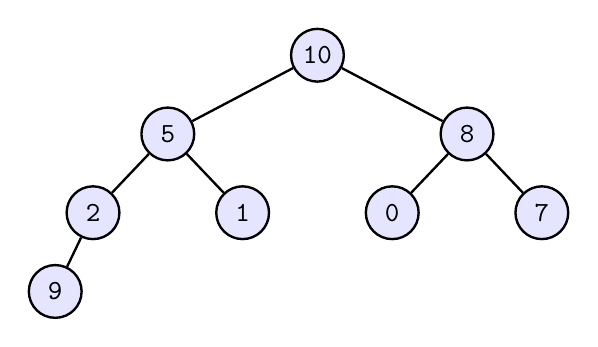
\begin{tikzpicture}

\fill[blue!10] (0.0, 0.0) circle (0.35);
\node [line width=0.03cm,black,minimum size=0.6699999999999999cm,draw,circle] at (0.0,0.0)(10){};\draw (0.0, 0.0) node[color=black] {\texttt{10}};
\fill[blue!10] (-1.9, -1.0) circle (0.35);
\node [line width=0.03cm,black,minimum size=0.6699999999999999cm,draw,circle] at (-1.9,-1.0)(5){};\draw (-1.9, -1.0) node[color=black] {\texttt{5}};
\fill[blue!10] (1.9, -1.0) circle (0.35);
\node [line width=0.03cm,black,minimum size=0.6699999999999999cm,draw,circle] at (1.9,-1.0)(8){};\draw (1.9, -1.0) node[color=black] {\texttt{8}};
\fill[blue!10] (-2.85, -2.0) circle (0.35);
\node [line width=0.03cm,black,minimum size=0.6699999999999999cm,draw,circle] at (-2.85,-2.0)(2){};\draw (-2.85, -2.0) node[color=black] {\texttt{2}};
\fill[blue!10] (-0.95, -2.0) circle (0.35);
\node [line width=0.03cm,black,minimum size=0.6699999999999999cm,draw,circle] at (-0.95,-2.0)(1){};\draw (-0.95, -2.0) node[color=black] {\texttt{1}};
\fill[blue!10] (0.95, -2.0) circle (0.35);
\node [line width=0.03cm,black,minimum size=0.6699999999999999cm,draw,circle] at (0.95,-2.0)(0){};\draw (0.95, -2.0) node[color=black] {\texttt{0}};
\fill[blue!10] (2.85, -2.0) circle (0.35);
\node [line width=0.03cm,black,minimum size=0.6699999999999999cm,draw,circle] at (2.85,-2.0)(7){};\draw (2.85, -2.0) node[color=black] {\texttt{7}};
\fill[blue!10] (-3.33, -3.0) circle (0.35);
\node [line width=0.03cm,black,minimum size=0.6699999999999999cm,draw,circle] at (-3.33,-3.0)(9){};\draw (-3.33, -3.0) node[color=black] {\texttt{9}};\draw[line width=0.03cm,black] (10) to  (5);
\draw[line width=0.03cm,black] (10) to  (8);
\draw[line width=0.03cm,black] (5) to  (2);
\draw[line width=0.03cm,black] (5) to  (1);
\draw[line width=0.03cm,black] (8) to  (0);
\draw[line width=0.03cm,black] (8) to  (7);
\draw[line width=0.03cm,black] (2) to  (9);
\end{tikzpicture}

\end{center}



It's easy to see that in the DFA, the $a$--
and $b$--transitions from the state $\{\}$ goes back to itself.
Therefore the completed DFA is this:


\begin{center}
\begin{tikzpicture}[>=triangle 60,shorten >=0.5pt,node distance=2cm,auto,initial text=, double distance=2pt]
\node[state,initial] (A) at (  0,  0) {$\{q_0\}$};
\node[state] (B) at (  3,  0) {$\{\}$};

\path[->]
(A) edge [bend left=0,pos=0.5,above] node {$a,b$} (B)
(B) edge [loop above] node {$a,b$} ()

;
\end{tikzpicture}
\end{center}
    



\newpage

Solution to Exercise \ref{ex:dfa-as-powerful-as-nfa1}\labeltext{}{sol:dfa-as-powerful-as-nfa1}.

\tinysidebar{\debug{exercises/{dfa-as-powerful-as-nfa1/answer.tex}}}

    Solution not provided.
    

\newpage

Solution to Exercise \ref{ex:dfa-as-powerful-as-nfa2}\labeltext{}{sol:dfa-as-powerful-as-nfa2}.

\tinysidebar{\debug{exercises/{dfa-as-powerful-as-nfa2/answer.tex}}}

    Solution not provided.
    

\newpage

Solution to Exercise \ref{ex:dfa-as-powerful-as-nfa3}\labeltext{}{sol:dfa-as-powerful-as-nfa3}.

\tinysidebar{\debug{exercises/{dfa-as-powerful-as-nfa3/answer.tex}}}

    Solution not provided.
    

\newpage

Solution to Exercise \ref{ex:dfa-as-powerful-as-nfa4}\labeltext{}{sol:dfa-as-powerful-as-nfa4}.

\tinysidebar{\debug{exercises/{dfa-as-powerful-as-nfa4/answer.tex}}}

    Solution not provided.
    

\newpage

Solution to Exercise \ref{ex:closure0}\labeltext{}{sol:closure0}.

\tinysidebar{\debug{exercises/{closure0/answer.tex}}}

    Solution not provided.
    

\newpage

Solution to Exercise \ref{ex:closure1}\labeltext{}{sol:closure1}.

\tinysidebar{\debug{exercises/{closure1/answer.tex}}}

    Solution not provided.
    

\newpage

Solution to Exercise \ref{ex:closure2}\labeltext{}{sol:closure2}.

\tinysidebar{\debug{exercises/{closure2/answer.tex}}}

    Solution not provided.
    

\newpage

Solution to Exercise \ref{ex:closure3}\labeltext{}{sol:closure3}.

\tinysidebar{\debug{exercises/{closure3/answer.tex}}}

    Solution not provided.
    

\newpage

Solution to Exercise \ref{ex:closure4}\labeltext{}{sol:closure4}.

\tinysidebar{\debug{exercises/{closure4/answer.tex}}}

    Solution not provided.
    

\newpage

Solution to Exercise \ref{ex:closure5}\labeltext{}{sol:closure5}.

\tinysidebar{\debug{exercises/{closure5/answer.tex}}}

    Solution not provided.
    

\newpage

Solution to Exercise \ref{ex:closure6}\labeltext{}{sol:closure6}.

\tinysidebar{\debug{exercises/{closure6/answer.tex}}}

    Solution not provided.
    

\newpage

Solution to Exercise \ref{ex:closure7}\labeltext{}{sol:closure7}.

\tinysidebar{\debug{exercises/{closure7/answer.tex}}}

    Solution not provided.
    

\newpage

Solution to Exercise \ref{ex:closure8}\labeltext{}{sol:closure8}.

\tinysidebar{\debug{exercises/{closure8/answer.tex}}}

    Solution not provided.
    

\newpage

Solution to Exercise \ref{ex:closure9}\labeltext{}{sol:closure9}.

\tinysidebar{\debug{exercises/{closure9/answer.tex}}}

    Solution not provided.
    

\newpage

Solution to Exercise \ref{ex:closure10}\labeltext{}{sol:closure10}.

\tinysidebar{\debug{exercises/{closure10/answer.tex}}}

    Solution not provided.
    

\newpage

Solution to Exercise \ref{ex:closure11}\labeltext{}{sol:closure11}.

\tinysidebar{\debug{exercises/{closure11/answer.tex}}}

    Solution not provided.
    

\newpage

Solution to Exercise \ref{ex:closure12}\labeltext{}{sol:closure12}.

\tinysidebar{\debug{exercises/{closure12/answer.tex}}}

    Solution not provided.
    

